\documentclass[12pt,a4paper]{article}
\usepackage{amsmath, amssymb}
\usepackage{geometry}
\usepackage{hyperref}
\usepackage{booktabs}
\usepackage{graphicx}
\usepackage{setspace}
\usepackage{float}
\usepackage{xcolor}
\usepackage{tikz}
\usepackage{pgfplots}
\usepackage{listings}
\usepackage{array}
\usepackage{tabularx}
\usepackage{enumitem}
\usepackage{caption}
\usepackage{subcaption}
\usetikzlibrary{positioning,arrows.meta,shapes.geometric,fit,backgrounds,calc,decorations.pathreplacing}
\pgfplotsset{compat=1.18}
\graphicspath{{assets/}}

\geometry{margin=1in}
\setstretch{1.15}
\hypersetup{colorlinks=true, linkcolor=black, urlcolor=blue!60!black, citecolor=black}
\captionsetup{font=small, skip=4pt}
\setlength{\abovecaptionskip}{4pt}

% colours used in diagrams
\definecolor{cShell}{HTML}{DCE8F5}
\definecolor{cKern}{HTML}{E3F1DF}
\definecolor{cStore}{HTML}{FBEBD5}
\definecolor{cSync}{HTML}{EFE3F3}
\definecolor{jA}{HTML}{8DB6DD}
\definecolor{jB}{HTML}{F2B880}
\definecolor{jC}{HTML}{9FCF95}
\definecolor{codebg}{HTML}{F7F7F7}

\lstset{
  language=C, basicstyle=\ttfamily\scriptsize, backgroundcolor=\color{codebg},
  keywordstyle=\color{blue!60!black}\bfseries, commentstyle=\color{green!40!black}\itshape,
  stringstyle=\color{red!50!black}, numbers=left, numberstyle=\tiny\color{gray},
  frame=single, rulecolor=\color{gray!40}, breaklines=true, showstringspaces=false,
  tabsize=4, columns=fullflexible, keepspaces=true, xleftmargin=1.5em, framexleftmargin=1.5em,
  aboveskip=4pt, belowskip=4pt
}

\tikzset{
  box/.style={draw, rounded corners=2pt, align=center, font=\small, inner sep=5pt},
  arr/.style={-{Stealth[length=2.2mm]}, thick},
  darr/.style={-{Stealth[length=2.2mm]}, thick, dashed}
}

\begin{document}

% ================= TITLE PAGE =================
\begin{titlepage}
    \centering

    \Huge
    \textbf{Jaypee Institute of Information Technology, Sector - 62, Noida } \\
    \vspace{0.5cm}
    \Large
    \textbf{B.Tech CSE V Semester}\\
    \vspace{1cm}

    
\includegraphics[width=2.22in]{jiit_logo}\\

    \vspace{1cm}
    \Huge
    \textbf{Operating Systems Lab PBL Report}\\
    \Large

    \textbf{toyOS: A Miniature Operating System in User Space}\\
    \vspace{1cm}

    \Large
    \textbf{Submitted to}\\
    Dr. Prakash Kumar\\
    Dr. Vikash\\
    Ms. Sonal Saurabh\\[0.5cm]

    \textbf{Submitted by}
    \vspace{0.5cm}

    \begin{tabular}{lll}
        Harsh Sharma      & 2401030232 & B5 \\
        Karvy Singh       & 2401030234 & B5 \\
        Rudra Kumar Singh & 2401030237 & B5 \\
    \end{tabular}

    \vspace*{\fill}
    \normalsize
\end{titlepage}

{\singlespacing\tableofcontents}
\newpage

% ================= 1. TITLE =================
\section{Title of the Project}

\begin{center}
\Large\textbf{toyOS: A Miniature Operating System in User Space}\\[0.2em]
\normalsize\textit{A shell, CPU scheduler, memory manager, synchronization and deadlock layer,\\ disk scheduler and file system, running together as one Linux program}
\end{center}

% ================= 2. TEAM =================
\section{Details of the Team}

Every member owns one source file containing two modules (Table~\ref{tab:team}).

\begin{table}[H]
\centering
\caption{Team members, module ownership and lines of code}
\label{tab:team}
\small
\begin{tabular}{@{}llcllr@{}}
\toprule
\textbf{Name} & \textbf{Roll No.} & \textbf{Batch} & \textbf{Modules} & \textbf{File} & \textbf{Lines} \\
\midrule
Harsh Sharma      & 2401030232 & B5 & M1 Shell, M2 Memory & \texttt{main.c} & 486 \\
Karvy Singh       & 2401030234 & B5 & M3 CPU, M4 Sync./Deadlock & \texttt{kernel.c} & 440 \\
Rudra Kumar Singh & 2401030237 & B5 & M5 Disk, M6 Cache + FS & \texttt{fs.c} & 467 \\
\midrule
\multicolumn{4}{@{}l}{Shared header (data structures and interfaces)} & \texttt{toyos.h} & 96 \\
\multicolumn{5}{@{}l}{\textbf{Total}} & \textbf{1489} \\
\bottomrule
\end{tabular}
\end{table}

% ================= 3. ABSTRACT =================
\section{Abstract}

Operating systems are usually taught one topic at a time, for example a CPU scheduling program that prints a Gantt chart from a fixed table of burst times. In a real operating system these parts depend on each other: the scheduler decides which process runs, that process asks the file system for data, the request waits in a disk queue, and semaphores keep everything consistent.

In this project we built \textbf{toyOS}, a small but complete operating system that runs as one program on Linux and is written in about 1500 lines of C. Its shell supports background jobs, pipes and redirection. Every command runs as a job with its own Process Control Block and stack, and jobs are switched by our own scheduler (FCFS, SJF, Priority, Round Robin, MLFQ) using real context switches driven by a timer interrupt. Memory is allocated with first, next, best or worst fit, and page replacement (FIFO, LRU, OPT) can be studied on reference strings. A separate disk thread serves requests from a virtual disk with six disk scheduling algorithms, behind a page cache using FIFO, LRU or CLOCK, and an inode-based file system stores files persistently.

Our own semaphores solve the producer--consumer, readers--writers and dining philosophers problems. Deadlocks are handled by prevention, avoidance (Banker's algorithm), detection (wait-for graph) and recovery. Waiting, response and turnaround times, page faults and head movement are measured, so the algorithms can be compared on real workloads.

% ================= 4. SCOPE =================
\section{Scope of the Project}

toyOS covers all eight modules of the course syllabus in one system. Like xv6 or Minix it is a teaching OS: it runs its own built-in programs, not arbitrary Linux binaries, and all statistics are measured, not calculated from tables.

\subsection{Functional Requirements}
\begin{enumerate}[label=\textbf{FR\arabic*}, leftmargin=3.2em, itemsep=0pt, topsep=2pt]
    \item The shell shall run jobs in the foreground or background, connect them with pipes, support \texttt{<}, \texttt{>}, \texttt{>>}, history and \texttt{jobs}/\texttt{fg}.
    \item The kernel shall keep a PCB per job, show its state (New, Ready, Running, Blocked, Disk-wait, Sleeping) with \texttt{ps}, and allow \texttt{kill}.
    \item The CPU scheduler shall support FCFS, SJF, Priority (with aging), Round Robin and MLFQ, and report a Gantt chart with waiting, response and turnaround times.
    \item The memory manager shall allocate memory with first, next, best or worst fit, show holes and fragmentation, and simulate FIFO, LRU and OPT page replacement.
    \item Semaphores shall be used for pipes (producer--consumer), files (readers--writers) and the dining philosophers.
    \item Deadlock shall be prevented (resource ordering), avoided (Banker's algorithm), detected (wait-for graph) and recovered from (\texttt{kill}).
    \item The disk thread shall serve requests with FCFS, SSTF, SCAN, C-SCAN, LOOK or C-LOOK and report head movement.
    \item The file system shall store files persistently using inodes with direct and indirect blocks, behind a FIFO/LRU/CLOCK page cache, with \texttt{fsck} to check it.
\end{enumerate}

\subsection{Non-functional Requirements}
\begin{enumerate}[label=\textbf{NFR\arabic*}, leftmargin=3.6em, itemsep=0pt, topsep=2pt]
    \item \textbf{Portability:} builds with GCC and \texttt{make} on any Linux system, with no external libraries.
    \item \textbf{Readability:} about 1500 lines of plain C in clearly marked modules.
    \item \textbf{Responsiveness:} the shell stays usable while background jobs run.
    \item \textbf{Consistency:} kernel data is changed only with interrupts disabled; files survive restarts.
\end{enumerate}

\subsection{Modules of the Project}
\begin{enumerate}[label=\textbf{M\arabic*}, leftmargin=2.8em, itemsep=0pt, topsep=2pt]
    \item \textbf{Shell and user programs:} parsing, pipes, redirection, history and 19 programs (\texttt{cat}, \texttt{grep}, \texttt{sort}, \ldots).
    \item \textbf{Memory manager:} contiguous allocation with four fit policies and a page replacement simulator.
    \item \textbf{Processes and CPU scheduling:} PCB, states, context switching, timer interrupt, five policies.
    \item \textbf{Synchronization and deadlock:} semaphores, bounded buffers, Banker's algorithm, wait-for graph.
    \item \textbf{Disk scheduling:} a POSIX thread acting as disk controller with six algorithms.
    \item \textbf{Page cache and file system:} block cache, inodes with an indirect block, readers--writers locks, \texttt{fsck}.
\end{enumerate}

% ================= 5. TOOLS =================
\section{Tools and Technologies Used}

\begin{table}[H]
\centering
\caption{Tools and technologies}
\small
\begin{tabularx}{\textwidth}{@{}>{\raggedright\arraybackslash}p{6.2cm}X@{}}
\toprule
\textbf{Tool / API} & \textbf{Use in toyOS} \\
\midrule
C (C11), GCC, GNU Make, Linux & Language, compiler, build, host operating system \\
\texttt{getcontext}, \texttt{makecontext}, \texttt{swapcontext} & Jobs with their own stacks; context switching \\
\texttt{setitimer} + \texttt{SIGALRM} & Timer interrupt that ends a time quantum \\
\texttt{sigprocmask} & ``Disabling interrupts'' inside the kernel \\
POSIX threads, mutex, condition variable & Disk controller thread and its request queue \\
\texttt{pthread\_kill} + \texttt{SIGUSR1} & ``I/O complete'' interrupt from disk to CPU \\
\texttt{pread} / \texttt{pwrite} on \texttt{disk.img} & The virtual 1~MB disk \\
Git, GitHub; \LaTeX, TikZ, PGFPlots & Version control; this report and its diagrams \\
\bottomrule
\end{tabularx}
\end{table}

% ================= 6. DESIGN =================
\section{Design of the Project}

\subsection{System Architecture}

toyOS runs inside one Linux process (Figure~\ref{fig:arch}). The \emph{main thread} plays the role of the CPU: it runs the kernel (scheduler loop) and, in between, the jobs. A second POSIX thread plays the role of the \emph{disk controller}. Jobs enter the kernel only through system calls.

\begin{figure}[H]
\centering
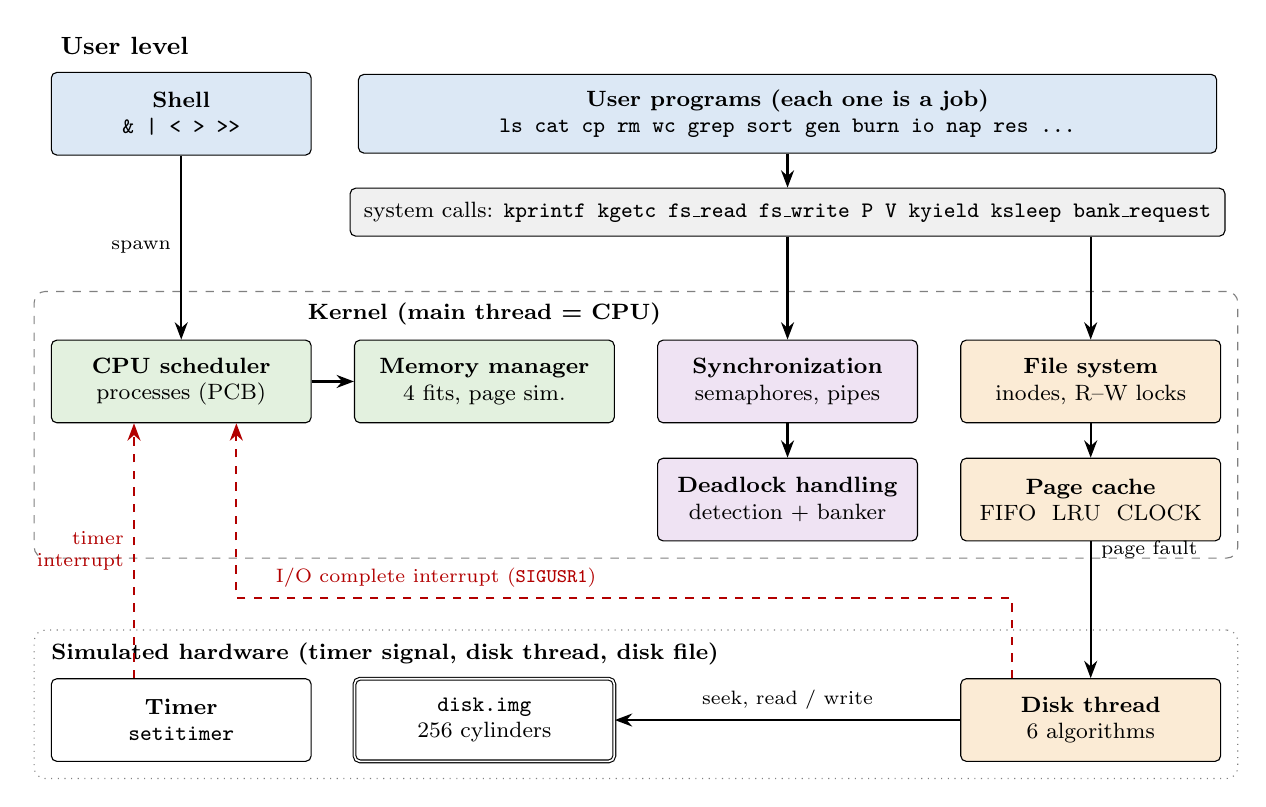
\begin{tikzpicture}[x=1cm, y=1cm, b/.style={box, font=\footnotesize, minimum width=3.3cm, minimum height=1.05cm}]
  \def\ca{1.7} \def\cb{5.55} \def\cc{9.4} \def\cd{13.25}
  % user level
  \node[b, fill=cShell] (sh) at (\ca,0) {\textbf{Shell}\\\texttt{\& | < > >>}};
  \node[box, font=\footnotesize, fill=cShell, minimum width=10.9cm, minimum height=1.0cm] (progs) at (\cc,0) {\textbf{User programs (each one is a job)}\\ \texttt{ls cat cp rm wc grep sort gen burn io nap res \ldots}};
  \node[box, font=\footnotesize, fill=gray!12, minimum width=10.9cm] (sys) at (\cc,-1.25) {system calls: \texttt{kprintf kgetc fs\_read fs\_write P V kyield ksleep bank\_request}};
  % kernel
  \node[b, fill=cKern] (sched) at (\ca,-3.4) {\textbf{CPU scheduler}\\processes (PCB)};
  \node[b, fill=cKern] (mem) at (\cb,-3.4) {\textbf{Memory manager}\\4 fits, page sim.};
  \node[b, fill=cSync] (sync) at (\cc,-3.4) {\textbf{Synchronization}\\semaphores, pipes};
  \node[b, fill=cStore] (fs) at (\cd,-3.4) {\textbf{File system}\\inodes, R--W locks};
  \node[b, fill=cSync] (dl) at (\cc,-4.9) {\textbf{Deadlock handling}\\detection + banker};
  \node[b, fill=cStore] (cache) at (\cd,-4.9) {\textbf{Page cache}\\FIFO\ \ LRU\ \ CLOCK};
  % hardware
  \node[b, fill=white] (timer) at (\ca,-7.7) {\textbf{Timer}\\\texttt{setitimer}};
  \node[b, fill=cStore] (dt) at (\cd,-7.7) {\textbf{Disk thread}\\6 algorithms};
  \node[b, fill=white, double] (img) at (\cb,-7.7) {\texttt{disk.img}\\256 cylinders};
  \begin{scope}[on background layer]
    \coordinate (ktop) at ($(sched.north)+(0,0.4)$);
    \coordinate (htop) at ($(timer.north)+(0,0.4)$);
    \node[draw=gray, dashed, rounded corners, fit=(sched)(fs)(dl)(cache)(ktop), inner sep=6pt] (kf) {};
    \node[draw=gray, dotted, rounded corners, fit=(timer)(dt)(img)(htop), inner sep=6pt] (hf) {};
  \end{scope}
  \node[font=\small\bfseries, anchor=south west] at ($(sh.north west)+(0,0.1)$) {User level};
  \node[font=\footnotesize\bfseries, anchor=north] at ($(kf.north -| mem)+(0,-0.03)$) {Kernel (main thread = CPU)};
  \node[font=\footnotesize\bfseries, anchor=north west] at ($(hf.north west)+(0.1,-0.05)$) {Simulated hardware (timer signal, disk thread, disk file)};
  \draw[arr] (sh) -- node[left, font=\scriptsize]{spawn} (sched);
  \draw[arr] (progs) -- (sys);
  \draw[arr] (sys.south -| sync) -- (sync);
  \draw[arr] (sys.south -| fs) -- (fs);
  \draw[arr] (sched) -- (mem);
  \draw[arr] (sync) -- (dl);
  \draw[arr] (fs) -- (cache);
  \draw[arr] (cache) -- node[right, font=\scriptsize]{page fault} (kf.south -| cache) -- (dt);
  \draw[arr] (dt) -- node[above, font=\scriptsize]{seek, read / write} (img);
  \draw[darr, red!70!black] ($(timer.north)+(-0.6,0)$) -- node[left, font=\scriptsize, align=right]{timer\\interrupt} ($(sched.south)+(-0.6,0)$);
  \draw[darr, red!70!black] ($(dt.north)+(-1.0,0)$) |- ($(kf.south)+(0,-0.5)$) -| node[pos=0.25, above, font=\scriptsize]{I/O complete interrupt (\texttt{SIGUSR1})} ($(sched.south)+(0.7,0)$);
\end{tikzpicture}
\caption{Architecture of toyOS. Dashed red arrows are interrupts (signals).}
\label{fig:arch}
\end{figure}

\begin{figure}[H]
\centering
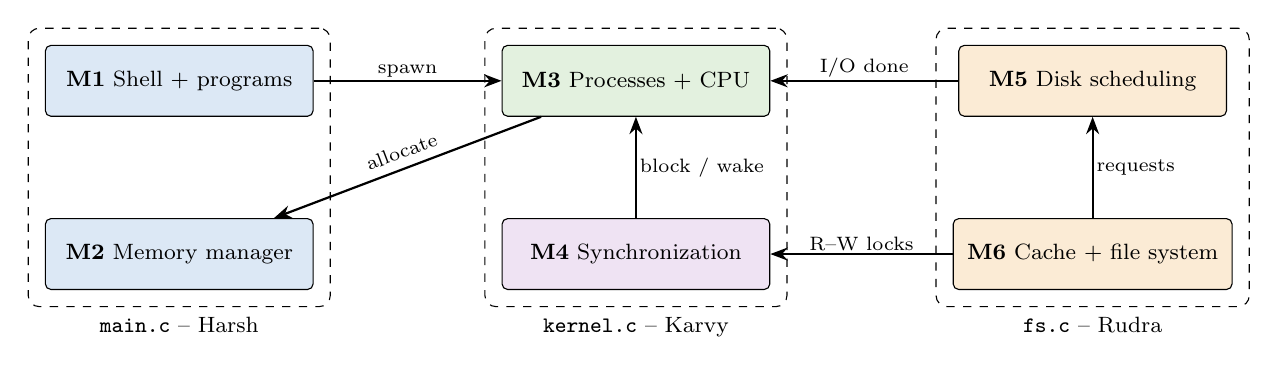
\begin{tikzpicture}[x=1cm, y=1cm, m/.style={box, minimum width=3.4cm, minimum height=0.9cm, font=\footnotesize}]
  \node[m, fill=cShell] (m1) at (0,0) {\textbf{M1} Shell + programs};
  \node[m, fill=cShell] (m2) at (0,-2.2) {\textbf{M2} Memory manager};
  \node[m, fill=cKern] (m3) at (5.8,0) {\textbf{M3} Processes + CPU};
  \node[m, fill=cSync] (m4) at (5.8,-2.2) {\textbf{M4} Synchronization};
  \node[m, fill=cStore] (m5) at (11.6,0) {\textbf{M5} Disk scheduling};
  \node[m, fill=cStore] (m6) at (11.6,-2.2) {\textbf{M6} Cache + file system};
  \node[draw, dashed, rounded corners, fit=(m1)(m2), inner sep=6pt, label={[font=\footnotesize]below:\texttt{main.c} -- Harsh}] {};
  \node[draw, dashed, rounded corners, fit=(m3)(m4), inner sep=6pt, label={[font=\footnotesize]below:\texttt{kernel.c} -- Karvy}] {};
  \node[draw, dashed, rounded corners, fit=(m5)(m6), inner sep=6pt, label={[font=\footnotesize]below:\texttt{fs.c} -- Rudra}] {};
  \draw[arr] (m1) -- node[above, font=\scriptsize, fill=white, inner sep=1pt]{spawn} (m3);
  \draw[arr] (m3) -- node[above, font=\scriptsize, sloped]{allocate} (m2);
  \draw[arr] (m5) -- node[above, font=\scriptsize, fill=white, inner sep=1pt]{I/O done} (m3);
  \draw[arr] (m6) -- node[right, font=\scriptsize, fill=white, inner sep=1pt]{requests} (m5);
  \draw[arr] (m6) -- node[above, font=\scriptsize, fill=white, inner sep=1pt]{R--W locks} (m4);
  \draw[arr] (m4) -- node[right, font=\scriptsize, fill=white, inner sep=1pt]{block / wake} (m3);
\end{tikzpicture}
\caption{The six modules, their files and owners, and how they use each other.}
\end{figure}

\subsection{Processes, States and Context Switching}

Every job has a PCB holding its saved context (\texttt{ucontext\_t}), memory block, priority, MLFQ level, SJF estimate, timing data, pipes and redirections, the semaphore or disk request it waits on, and its Banker's claim and allocation. Jobs move between the states of Figure~\ref{fig:states}. The kernel always runs with the timer signal blocked and a job runs with it unblocked; when the quantum ends, the \texttt{SIGALRM} handler runs on the job's stack and switches back to the kernel, exactly like a hardware timer interrupt followed by a context switch.

\begin{figure}[H]
\centering
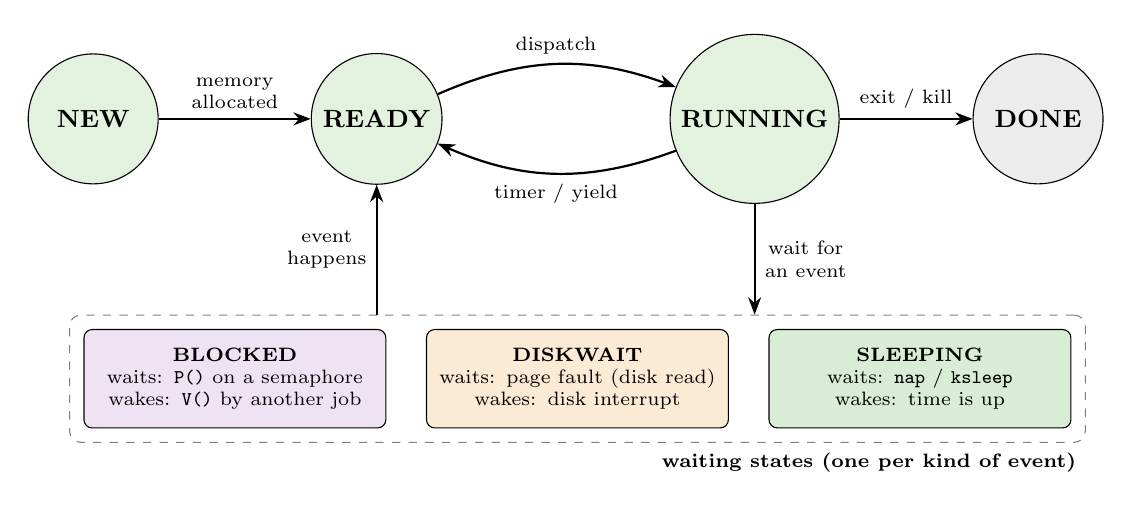
\begin{tikzpicture}[x=1cm, y=1cm, st/.style={draw, circle, minimum size=1.65cm, align=center, font=\small\bfseries, fill=cKern},
    ws/.style={draw, rounded corners=3pt, text width=3.6cm, minimum height=1.25cm, align=center, font=\scriptsize}, lbl/.style={font=\scriptsize, align=center}]
  \node[st] (new) at (0,0) {NEW};
  \node[st] (ready) at (3.6,0) {READY};
  \node[st] (run) at (8.4,0) {RUNNING};
  \node[st, fill=gray!15] (done) at (12,0) {DONE};
  \node[ws, fill=cSync] (blk) at (1.8,-3.3) {\textbf{BLOCKED}\\waits: \texttt{P()} on a semaphore\\wakes: \texttt{V()} by another job};
  \node[ws, fill=cStore] (dw) at (6.15,-3.3) {\textbf{DISKWAIT}\\waits: page fault (disk read)\\wakes: disk interrupt};
  \node[ws, fill=jC!40] (sl) at (10.5,-3.3) {\textbf{SLEEPING}\\waits: \texttt{nap} / \texttt{ksleep}\\wakes: time is up};
  \node[draw=gray, dashed, rounded corners, fit=(blk)(dw)(sl), inner sep=5pt, label={[font=\scriptsize\bfseries, anchor=north east]south east:waiting states (one per kind of event)}] (wait) {};
  \draw[arr] (new) -- node[above, lbl]{memory\\allocated} (ready);
  \draw[arr] (ready) to[bend left=22] node[above, lbl]{dispatch} (run);
  \draw[arr] (run) to[bend left=22] node[below, lbl]{timer / yield} (ready);
  \draw[arr] (run) -- node[above, lbl]{exit / kill} (done);
  \draw[arr] (run) -- node[right, lbl]{wait for\\an event} (run |- wait.north);
  \draw[arr] (ready |- wait.north) -- node[left, lbl]{event\\happens} (ready);
\end{tikzpicture}
\caption{Process state diagram as implemented in toyOS.}
\label{fig:states}
\end{figure}

\begin{figure}[H]
\centering
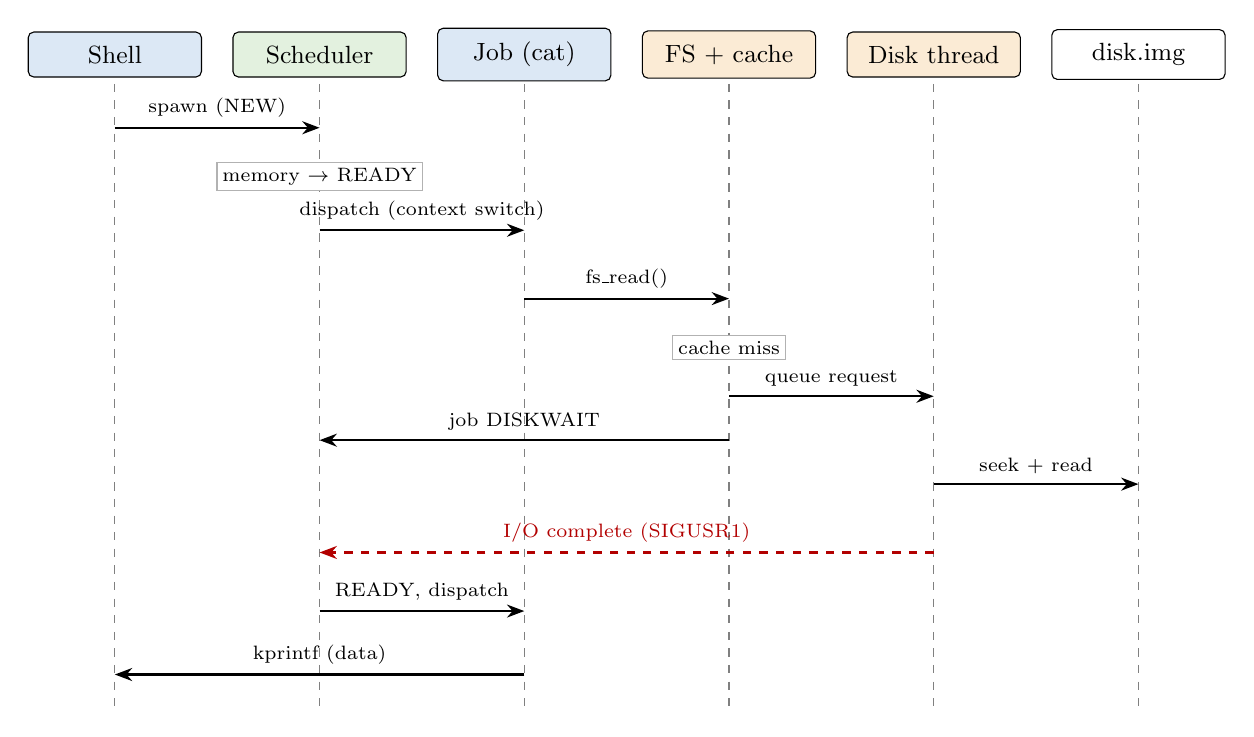
\begin{tikzpicture}[x=1cm, y=-0.62cm]
  \foreach \x/\n/\c in {0/Shell/cShell, 2.6/Scheduler/cKern, 5.2/Job (cat)/cShell, 7.8/FS + cache/cStore, 10.4/Disk thread/cStore, 13.0/disk.img/white}{
    \node[box, fill=\c, minimum width=2.2cm] at (\x,0) {\n};
    \draw[gray, dashed] (\x,0.6) -- (\x,13.4);
  }
  \newcommand{\msg}[4]{\draw[arr] (#1,#3) -- node[above, font=\scriptsize]{#4} (#2,#3);}
  \msg{0}{2.6}{1.5}{spawn (NEW)}
  \node[font=\scriptsize, fill=white, draw=gray!60, inner sep=2pt] at (2.6,2.5) {memory $\rightarrow$ READY};
  \msg{2.6}{5.2}{3.6}{dispatch (context switch)}
  \msg{5.2}{7.8}{5.0}{fs\_read()}
  \node[font=\scriptsize, fill=white, draw=gray!60, inner sep=2pt] at (7.8,6.0) {cache miss};
  \msg{7.8}{10.4}{7.0}{queue request}
  \draw[arr] (7.8,7.9) -- node[above, font=\scriptsize]{job DISKWAIT} (2.6,7.9);
  \msg{10.4}{13.0}{8.8}{seek + read}
  \draw[arr, red!70!black, dashed] (10.4,10.2) -- node[above, font=\scriptsize]{I/O complete (SIGUSR1)} (2.6,10.2);
  \msg{2.6}{5.2}{11.4}{READY, dispatch}
  \draw[arr] (5.2,12.7) -- node[above, font=\scriptsize]{kprintf (data)} (0,12.7);
\end{tikzpicture}
\caption{Sequence diagram of \texttt{cat notes.txt} when the block is not in the page cache.}
\end{figure}

\subsection{CPU Scheduling}

The scheduler picks the ready job with the smallest key; ties go to the job that has waited longest.

\begin{table}[H]
\centering
\caption{How each policy chooses the next job}
\small
\begin{tabularx}{\textwidth}{@{}llX@{}}
\toprule
\textbf{Policy} & \textbf{Preemptive?} & \textbf{Rule} \\
\midrule
FCFS & No & Oldest job in the ready queue \\
SJF & No & Smallest predicted burst $\tau_{n+1} = \alpha\, t_n + (1-\alpha)\,\tau_n$, $\alpha = 0.5$, per command \\
Priority & Yes & Smallest priority number (\texttt{nice}); aging raises a job waiting over 500 ms \\
Round Robin & Yes & Oldest ready job; a preempted job goes to the back \\
MLFQ & Yes & 3 levels, quantum $q, 2q, 4q$; full quantum moves a job down; boost every second \\
\bottomrule
\end{tabularx}
\end{table}

\subsection{Memory Management}

Each job's memory is one contiguous block of a 160~KB array. The memory map is a list of segments; allocation splits a hole, freeing merges neighbouring holes, and a job that does not fit waits in the NEW state. Next fit continues searching from the last allocation. Figure~\ref{fig:mem} is the real map from Test~2. For virtual memory, \texttt{pagesim} runs FIFO, LRU and OPT on a reference string and prints the textbook frame table.

\begin{figure}[H]
\centering
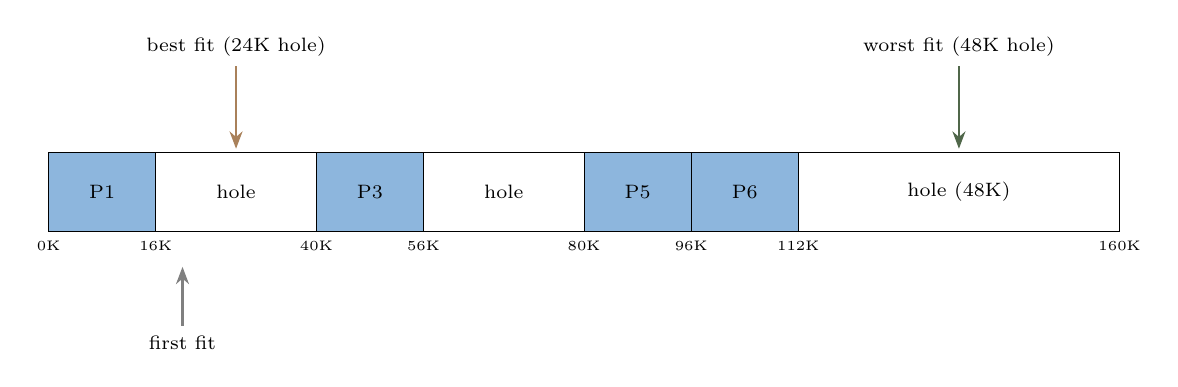
\begin{tikzpicture}[x=0.085cm]
  \foreach \s/\e/\l/\c in {0/16/P1/jA, 16/40/hole/white, 40/56/P3/jA, 56/80/hole/white, 80/96/P5/jA, 96/112/P6/jA, 112/160/hole (48K)/white}{
    \draw[fill=\c] (\s,0) rectangle (\e,1);
    \node[font=\scriptsize] at ({(\s+\e)/2},0.5) {\l};
    \node[font=\tiny, below] at (\s,0) {\s K};
  }
  \node[font=\tiny, below] at (160,0) {160K};
  \draw[arr, jB!70!black] (28,2.1) -- (28,1.05); \node[font=\scriptsize, above, align=center] at (28,2.1) {best fit (24K hole)};
  \draw[arr, jC!50!black] (136,2.1) -- (136,1.05); \node[font=\scriptsize, above, align=center] at (136,2.1) {worst fit (48K hole)};
  \draw[arr, gray] (20,-1.2) -- (20,-0.45); \node[font=\scriptsize, below] at (20,-1.2) {first fit};
\end{tikzpicture}
\caption{Memory map with three holes (96K free, largest 48K, 50\% external fragmentation) and where each policy places a new 16K job.}
\label{fig:mem}
\end{figure}

\subsection{Synchronization and Deadlock Handling}

\texttt{P()} blocks a job in the BLOCKED state; \texttt{V()} hands the semaphore to the oldest waiter. Every pipe is a bounded buffer (Figure~\ref{fig:pipe}), every file has a readers--writers lock, and \texttt{philo} runs the dining philosophers. Table~\ref{tab:dl} shows how all four deadlock strategies of the syllabus appear in toyOS, and Figure~\ref{fig:wfg} is the wait-for graph found in Test~4.

\begin{figure}[H]
\centering
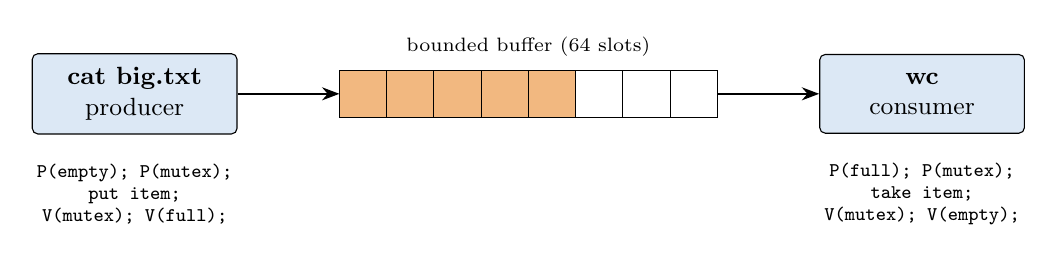
\begin{tikzpicture}
  \node[box, fill=cShell, minimum height=1cm, minimum width=2.6cm] (prod) at (0,0) {\textbf{cat big.txt}\\producer};
  \foreach \i in {0,...,7} \draw[fill=\ifnum\i<5 jB\else white\fi] (2.6+\i*0.6,-0.3) rectangle (3.2+\i*0.6,0.3);
  \node[font=\scriptsize] at (5.0,0.6) {bounded buffer (64 slots)};
  \node[box, fill=cShell, minimum height=1cm, minimum width=2.6cm] (cons) at (10,0) {\textbf{wc}\\consumer};
  \draw[arr] (prod) -- (2.6,0);
  \draw[arr] (7.4,0) -- (cons);
  \node[font=\scriptsize, align=center, below=0.25cm of prod] {\texttt{P(empty); P(mutex);}\\\texttt{put item;}\\\texttt{V(mutex); V(full);}};
  \node[font=\scriptsize, align=center, below=0.25cm of cons] {\texttt{P(full); P(mutex);}\\\texttt{take item;}\\\texttt{V(mutex); V(empty);}};
\end{tikzpicture}
\caption{The pipe \texttt{cat big.txt | wc} is a bounded buffer protected by three semaphores.}
\label{fig:pipe}
\end{figure}

\begin{table}[H]
\centering
\caption{Deadlock handling in toyOS}
\label{tab:dl}
\small
\begin{tabularx}{\textwidth}{@{}l>{\raggedright\arraybackslash}X@{}}
\toprule
\textbf{Strategy} & \textbf{Implementation} \\
\midrule
Prevention & \texttt{philo safe}: the last philosopher picks forks in reverse order, so circular wait cannot happen \\
Avoidance & Banker's algorithm: jobs (\texttt{res A B C}) declare a maximum claim; a request is granted only if the safety algorithm finds a safe sequence, otherwise the job waits \\
Detection & \texttt{deadlock}: edge P$\rightarrow$Q when P waits on a binary semaphore held by Q; a cycle is a deadlock \\
Recovery & \texttt{kill}: the job is terminated and all semaphores and resources it held are given back \\
\bottomrule
\end{tabularx}
\end{table}

\begin{figure}[H]
\centering
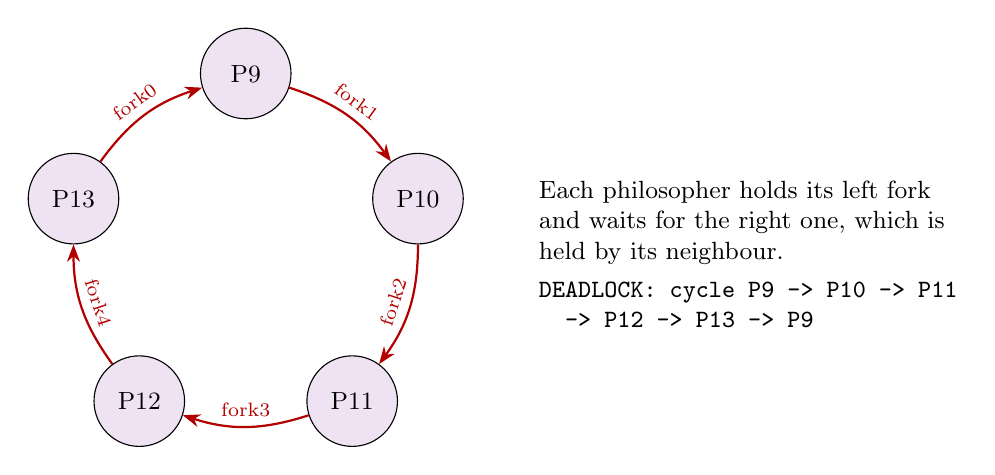
\begin{tikzpicture}
  \foreach \i/\p in {0/9,1/10,2/11,3/12,4/13} {
    \node[draw, circle, fill=cSync, minimum size=1.15cm, font=\small] (p\i) at ({90-72*\i}:2.3) {P\p};
  }
  \foreach \i/\j/\f in {0/1/fork1, 1/2/fork2, 2/3/fork3, 3/4/fork4, 4/0/fork0} {
    \draw[arr, red!70!black] (p\i) to[bend left=18] node[font=\scriptsize, sloped, above]{\f} (p\j);
  }
  \node[font=\small, align=left, anchor=west] at (3.6,0) {Each philosopher holds its left fork\\and waits for the right one, which is\\held by its neighbour.\\[0.3em]\texttt{DEADLOCK: cycle P9 -> P10 -> P11}\\\texttt{\ \ -> P12 -> P13 -> P9}};
\end{tikzpicture}
\caption{Wait-for graph of the dining philosophers deadlock found by the \texttt{deadlock} command.}
\label{fig:wfg}
\end{figure}

\subsection{Disk, Page Cache and File System}

\texttt{disk.img} has 2048 blocks of 512 bytes, 8 blocks per cylinder (256 cylinders). Block 0 is the superblock, block 1 the free-block bitmap, blocks 2--5 hold 32 inodes, 6--7 the directory and the rest data. An inode has 27 direct pointers and one indirect block of 256 pointers, so a file can be 141.5~KB (Figure~\ref{fig:inode}). Every block read goes through an 8-frame page cache (Figure~\ref{fig:cacheflow}); on a miss, the request joins the disk queue and the disk thread chooses the next request with the selected algorithm.

\begin{figure}[H]
\centering
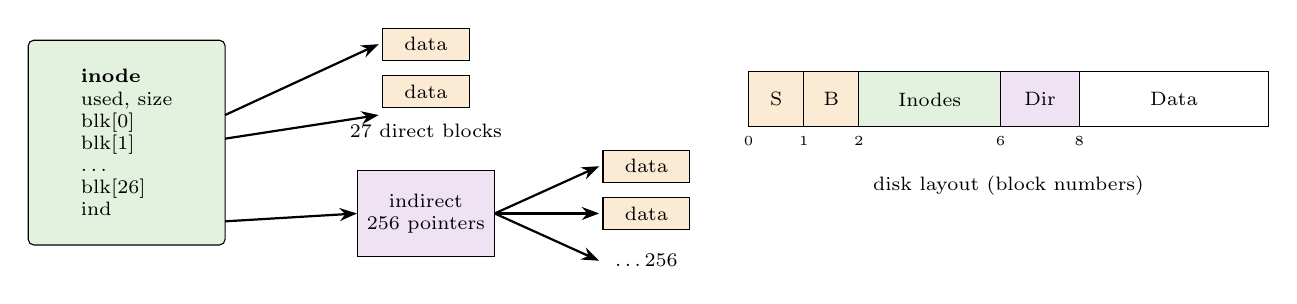
\begin{tikzpicture}[x=1cm, y=1cm]
  \node[box, fill=cKern, minimum width=2.5cm, minimum height=2.6cm, align=left, font=\scriptsize] (ino) at (0,0) {\textbf{inode}\\used, size\\blk[0]\\blk[1]\\\ldots\\blk[26]\\ind};
  \foreach \y/\n in {0.35/0, 0.05/1} \draw[arr] (1.25,\y) -- (3.2,\y+0.9-\n*0.6);
  \node[draw, fill=cStore, minimum width=1.1cm, font=\scriptsize] at (3.8,1.25) {data};
  \node[draw, fill=cStore, minimum width=1.1cm, font=\scriptsize] at (3.8,0.65) {data};
  \node[font=\scriptsize] at (3.8,0.15) {27 direct blocks};
  \node[draw, fill=cSync, minimum width=1.6cm, minimum height=1.1cm, font=\scriptsize, align=center] (ib) at (3.8,-0.9) {indirect\\256 pointers};
  \draw[arr] (1.25,-1.0) -- (ib.west);
  \foreach \y in {-0.3,-0.9,-1.5} \draw[arr] (ib.east) -- (6.0,\y);
  \foreach \y in {-0.3,-0.9} \node[draw, fill=cStore, minimum width=1.1cm, font=\scriptsize] at (6.6,\y) {data};
  \node[font=\scriptsize] at (6.6,-1.5) {\ldots 256};
  \begin{scope}[xshift=7.9cm, yshift=0.2cm]
    \foreach \s/\e/\l/\c in {0/0.7/S/cStore, 0.7/1.4/B/cStore, 1.4/3.2/Inodes/cKern, 3.2/4.2/Dir/cSync, 4.2/6.6/Data/white}{
      \draw[fill=\c] (\s,0) rectangle (\e,0.7); \node[font=\scriptsize] at ({(\s+\e)/2},0.35) {\l};}
    \foreach \b/\x in {0/0,1/0.7,2/1.4,6/3.2,8/4.2} \node[font=\tiny, below] at (\x,0) {\b};
    \node[font=\scriptsize, align=center] at (3.3,-0.75) {disk layout (block numbers)};
  \end{scope}
\end{tikzpicture}
\caption{An inode with direct and indirect blocks (left) and the layout of \texttt{disk.img} (right).}
\label{fig:inode}
\end{figure}

\begin{figure}[H]
\centering
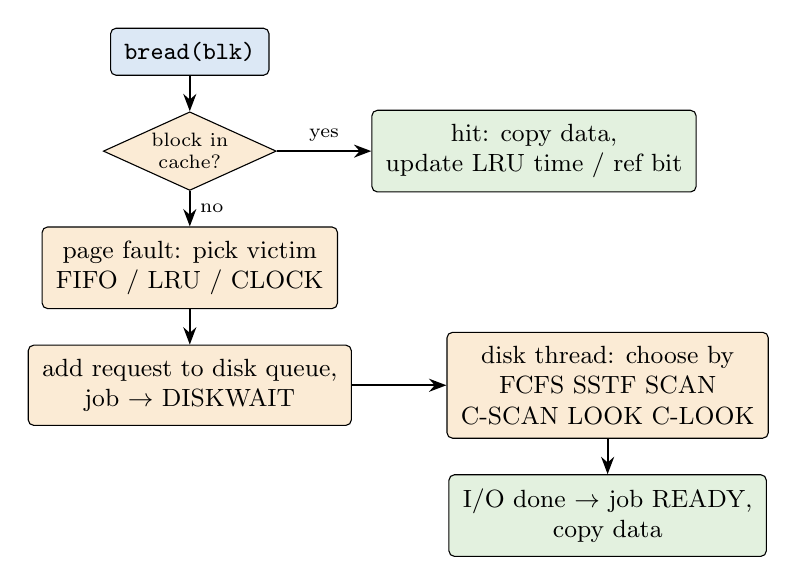
\begin{tikzpicture}[node distance=0.45cm and 0.8cm, dec/.style={draw, diamond, aspect=2.2, fill=cStore, font=\scriptsize, align=center, inner sep=1pt}]
  \node[box, fill=cShell] (s) {\texttt{bread(blk)}};
  \node[dec, below=of s] (hit) {block in\\cache?};
  \node[box, fill=cKern, right=1.2cm of hit] (h) {hit: copy data,\\update LRU time / ref bit};
  \node[box, fill=cStore, below=of hit] (v) {page fault: pick victim\\FIFO / LRU / CLOCK};
  \node[box, fill=cStore, below=of v] (q) {add request to disk queue,\\job $\rightarrow$ DISKWAIT};
  \node[box, fill=cStore, right=1.2cm of q] (d) {disk thread: choose by\\FCFS SSTF SCAN\\C-SCAN LOOK C-LOOK};
  \node[box, fill=cKern, below=of d] (w) {I/O done $\rightarrow$ job READY,\\copy data};
  \draw[arr] (s) -- (hit);
  \draw[arr] (hit) -- node[above, font=\scriptsize]{yes} (h);
  \draw[arr] (hit) -- node[right, font=\scriptsize]{no} (v);
  \draw[arr] (v) -- (q);
  \draw[arr] (q) -- (d);
  \draw[arr] (d) -- (w);
\end{tikzpicture}
\caption{Reading a block through the page cache and the disk scheduler.}
\label{fig:cacheflow}
\end{figure}

% ================= 7. IMPLEMENTATION =================
\section{Implementation Details}

toyOS has three source files, one per member, plus a shared header (Table~\ref{tab:team}): 1489 lines in total. It is built with \texttt{make} and started with \texttt{./toyos}; \texttt{help} lists all commands. The listings below are taken directly from the source.

\subsection{M1 and M2: Shell and Memory Manager (\texttt{main.c}, Harsh Sharma)}

The shell splits a line into words, removes the redirections \texttt{<}, \texttt{>}, \texttt{>>}, splits at every \texttt{|} and creates one job per part, joined by new pipes. Programs read input through one helper that works for files, pipes and \texttt{< file}. The memory manager implements the four fit policies:

\noindent\begin{minipage}{\linewidth}
\begin{lstlisting}[firstnumber=389, caption={First, next, best and worst fit (\texttt{main.c})}]
int mem_alloc(int size, int pid) {
    int b = -1, k0 = 0;
    if (mem_algo == NEXT)
        while (k0 < nsegs && segs[k0].start + segs[k0].size <= nextpos) k0++;
    for (int j = 0; j < nsegs; j++) {
        int i = (k0 + j) % nsegs;
        if (segs[i].pid || segs[i].size < size) continue;
        if (b < 0 || (mem_algo == BEST && segs[i].size < segs[b].size)
                  || (mem_algo == WORST && segs[i].size > segs[b].size)) b = i;
        if (mem_algo == FIRST || mem_algo == NEXT) break;
    }
    if (b < 0) return -1;
    nextpos = segs[b].start + size;
    nalloc++;
    if (segs[b].size > size) {
        memmove(&segs[b + 2], &segs[b + 1], (nsegs - b - 1) * sizeof(seg));
        segs[b + 1] = (seg){segs[b].start + size, segs[b].size - size, 0};
        segs[b].size = size; nsegs++;
    }
    segs[b].pid = pid;
    int used = 0;
    for (int i = 0; i < nsegs; i++) if (segs[i].pid) used += segs[i].size;
    if (used > peak) peak = used;
    return segs[b].start;
}
\end{lstlisting}
\end{minipage}

\subsection{M3 and M4: Scheduling and Synchronization (\texttt{kernel.c}, Karvy Singh)}

\texttt{dispatch} performs one context switch and, when the job comes back (timer, block, yield or exit), updates the CPU time, Gantt chart, MLFQ level and SJF estimate:

\noindent\begin{minipage}{\linewidth}
\begin{lstlisting}[firstnumber=144, caption={Dispatching a job (\texttt{kernel.c})}]
static void dispatch(pcb *p) {
    int q = (cpu_algo == FCFS || cpu_algo == SJF) ? 0 : cpu_algo == MLFQ ? quantum << p->level : quantum;
    struct timespec zero = {0, 0};
    p->trun = ms(); p->wait += p->trun - p->tready;
    p->state = RUNNING; cur = p;
    if (p->pid != lastpid) { nswitch++; lastpid = p->pid; }
    if (!p->tfirst) p->tfirst = p->trun;
    if (q) timer_set(q);
    swapcontext(&kctx, &p->ctx);
    timer_set(0);
    while (sigtimedwait(&intr, 0, &zero) > 0);
    cur = 0;
    long now = ms(), ran = now - p->trun;
    p->cpu += ran; p->burst += ran; busy += ran;
    if (ng && gantt[ng - 1].pid == p->pid) gantt[ng - 1].t1 = now;
    else if (ng < 512) { gantt[ng].pid = p->pid; gantt[ng].t0 = p->trun; gantt[ng++].t1 = now; }
    if (reason == R_PREEMPT || reason == R_YIELD) {
        if (reason == R_PREEMPT && cpu_algo == MLFQ && p->level < 2) p->level++;
        make_ready(p); return;
    }
    p->tau = alpha * p->burst + (1 - alpha) * p->tau;
    *tau_of(p->name) = p->tau; p->burst = 0;
    if (p->state == DONE) finish(p);
}
\end{lstlisting}
\end{minipage}

\noindent\begin{minipage}{\linewidth}
\begin{lstlisting}[firstnumber=395, caption={Banker's resource-request algorithm (\texttt{kernel.c})}]
int bank_request(int *req) {
    intr_off();
    for (int r = 0; r < NRES; r++)
        if (req[r] > cur->max[r] - cur->alloc[r]) { intr_on(); return -1; }
    for (;;) {
        int ok = 1;
        for (int r = 0; r < NRES; r++) if (req[r] > avail[r]) ok = 0;
        if (ok) {
            for (int r = 0; r < NRES; r++) { avail[r] -= req[r]; cur->alloc[r] += req[r]; }
            if (safe(0) >= 0) break;
            for (int r = 0; r < NRES; r++) { avail[r] += req[r]; cur->alloc[r] -= req[r]; }
            denied++;
        }
        cur->state = BLOCKED; cur->waiting = &bankq; cur->seq = ++seqno;
        to_kernel(R_BLOCK);
    }
    intr_on();
    return 0;
}
\end{lstlisting}
\end{minipage}

\subsection{M5 and M6: Disk, Cache and File System (\texttt{fs.c}, Rudra Kumar Singh)}

The disk thread waits on a condition variable, takes the request chosen below, sleeps for the seek time, performs the transfer and raises the I/O-complete interrupt. \texttt{disksim} runs the same function on a textbook request queue.

\noindent\begin{minipage}{\linewidth}
\begin{lstlisting}[firstnumber=33, caption={Disk scheduling: choosing the next request (\texttt{fs.c})}]
static int choose(void) {
    int b = 0;
    if (disk_algo == D_SSTF) b = nearest(0);
    else if (disk_algo == D_SCAN) {
        if ((b = nearest(dir)) < 0) {
            int edge = dir > 0 ? NCYL - 1 : 0;
            moved += abs(edge - head); head = edge; dir = -dir;
            b = nearest(dir);
        }
    } else if (disk_algo == D_CSCAN) {
        if ((b = nearest(1)) < 0) {
            moved += (NCYL - 1 - head) + (NCYL - 1);
            head = 0;
            b = nearest(1);
        }
    } else if (disk_algo == D_LOOK) {
        if ((b = nearest(dir)) < 0) {
            dir = -dir;
            b = nearest(dir);
        }
    } else if (disk_algo == D_CLOOK) {
        dir = 1;
        if ((b = nearest(1)) < 0)
            for (int i = b = 0; i < npend; i++)
                if (cyl(i) < cyl(b)) b = i;
    }
    return b;
}
\end{lstlisting}
\end{minipage}

% ================= 8. TESTING =================
\section{Testing Details}

Each test is a script in \texttt{tests/}, run as \texttt{./toyos < tests/<name>.txt}; the shell echoes every command, so the output is a full record. All numbers below come from these runs.

\begin{table}[H]
\centering
\caption{Test cases (all passed)}
\label{tab:tests}
\footnotesize
\renewcommand{\arraystretch}{1.15}
\setlength{\tabcolsep}{3.5pt}
\begin{tabularx}{\textwidth}{@{}p{0.75cm}p{0.8cm}>{\raggedright\arraybackslash}X>{\raggedright\arraybackslash}X@{}}
\toprule
\textbf{ID} & \textbf{Mod.} & \textbf{Input} & \textbf{Expected = actual result} \\
\midrule
TC1 & M1 M6 & \texttt{gen 40 > big.txt}; \texttt{wc}; \texttt{cat | wc}; \texttt{cp}; \texttt{rm} & 40 lines / 400 words both ways; copy same size; \texttt{rm} frees blocks \\
TC2 & M2 & 6 jobs, kill 2, new job under worst / best fit & Holes at 16K, 56K, 112K; worst fit uses 112K, best fit 16K; extra jobs wait in NEW \\
TC3 & M3 & \texttt{burn 4}, \texttt{burn 1}, \texttt{burn 2} under FCFS, SJF, RR & Avg.\ waiting 301 / 133 / 250 ms; RR response 50 ms (Fig.~\ref{fig:gantt}) \\
TC4 & M3 & \texttt{nice 7}, \texttt{nice 1}, \texttt{nice 4} under PRIO & Run in priority order 1, 4, 7 \\
TC5 & M3 & \texttt{burn 4} + \texttt{io 30} under MLFQ & I/O job response 20 ms, finishes in 204 ms \\
TC6 & M4 & \texttt{gen 200 | wc}; 2 readers + 1 writer & 200 lines through the pipe; writer waits on \texttt{file0.wrt} \\
TC7 & M4 & \texttt{philo}; \texttt{deadlock}; \texttt{kill 9}; \texttt{philo safe} & Cycle P9$\rightarrow$\ldots$\rightarrow$P13$\rightarrow$P9 found; kill recovers; safe version never deadlocks \\
TC8 & M4 & 5 \texttt{res} jobs, total (10, 5, 7) & Safe sequence P2 P4 P1 P3 P5; 1 unsafe request delayed; all finish \\
TC9 & M2 & \texttt{pagesim} on two reference strings & FIFO 15, LRU 12, OPT 9 faults; Belady: FIFO 9 faults (3 frames) vs 10 (4) \\
TC10 & M5 & 5 $\times$ \texttt{io 25} per algorithm; \texttt{disksim} & Measured and textbook head movement (Fig.~\ref{fig:disk}) \\
TC11 & M6 & Hot file between two 5-block files, 8 frames & LRU 21 faults; FIFO and CLOCK 23 \\
TC12 & M6 & 300-line file; \texttt{stat}; \texttt{fsck}; kill \texttt{cp} mid-write & Indirect block used; \texttt{fsck} clean; partial copy consistent \\
TC13 & M1 & \texttt{< > >> | grep head sort}, \texttt{nap}, \texttt{!10} & Correct output; \texttt{nap} SLEEPING with 0 ms CPU; history repeats \\
TC14 & M6 & Exit and restart, \texttt{ls} & Files from the previous run are present \\
\bottomrule
\end{tabularx}
\end{table}

\subsection{CPU Scheduling Results}

\newcommand{\gs}{0.019}
\newcommand{\gbar}[4]{\fill[#4] (#1*\gs,0) rectangle (#2*\gs,0.55); \draw (#1*\gs,0) rectangle (#2*\gs,0.55); \node[font=\scriptsize] at ({(#1+#2)/2*\gs},0.275) {#3};}
\newcommand{\gtick}[1]{\node[font=\tiny, below] at (#1*\gs,0) {#1};}

\begin{figure}[H]
\centering
\begin{tikzpicture}[x=1cm, y=1cm]
  \begin{scope}[yshift=2.2cm]
    \node[anchor=east, font=\small\bfseries] at (-0.2,0.3) {FCFS};
    \gbar{0}{400}{A}{jA}\gbar{400}{500}{B}{jB}\gbar{500}{700}{C}{jC}
    \foreach \t in {0,400,500,700} {\gtick{\t}}
  \end{scope}
  \begin{scope}[yshift=1.1cm]
    \node[anchor=east, font=\small\bfseries] at (-0.2,0.3) {SJF};
    \gbar{0}{100}{B}{jB}\gbar{100}{300}{C}{jC}\gbar{300}{700}{A}{jA}
    \foreach \t in {0,100,300,700} {\gtick{\t}}
  \end{scope}
  \begin{scope}[yshift=0cm]
    \node[anchor=east, font=\small\bfseries] at (-0.2,0.3) {RR};
    \gbar{0}{50}{A}{jA}\gbar{50}{100}{B}{jB}\gbar{100}{150}{C}{jC}\gbar{150}{200}{A}{jA}\gbar{200}{250}{B}{jB}
    \gbar{250}{300}{C}{jC}\gbar{300}{350}{A}{jA}\gbar{350}{400}{C}{jC}\gbar{400}{450}{A}{jA}\gbar{450}{500}{C}{jC}\gbar{500}{700}{A}{jA}
    \foreach \t in {0,100,200,300,400,500,700} {\gtick{\t}}
  \end{scope}
  \node[font=\scriptsize] at (6.65,-0.7) {time (ms) \quad A = \texttt{burn 4} (400 ms), B = \texttt{burn 1} (100 ms), C = \texttt{burn 2} (200 ms), quantum 50 ms};
\end{tikzpicture}
\caption{Gantt charts recorded by toyOS for the same three jobs (TC3).}
\label{fig:gantt}
\end{figure}

\begin{figure}[H]
\centering
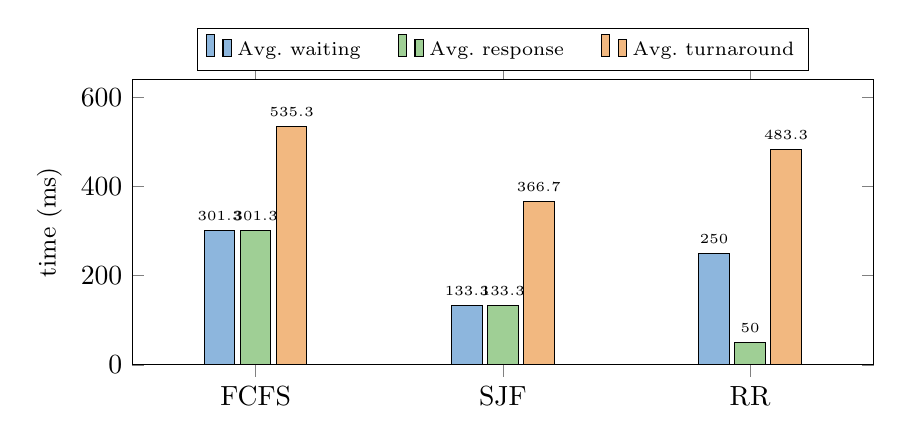
\begin{tikzpicture}
\begin{axis}[ybar, bar width=11pt, width=11cm, height=5.2cm, ymin=0, ymax=640,
  symbolic x coords={FCFS,SJF,RR}, xtick=data, ylabel={time (ms)}, ylabel style={font=\small},
  legend style={at={(0.5,1.03)}, anchor=south, legend columns=3, font=\scriptsize, /tikz/every even column/.append style={column sep=0.4cm}},
  nodes near coords, nodes near coords style={font=\tiny}, enlarge x limits=0.25]
\addplot[fill=jA] coordinates {(FCFS,301.3) (SJF,133.3) (RR,250)};
\addplot[fill=jC] coordinates {(FCFS,301.3) (SJF,133.3) (RR,50)};
\addplot[fill=jB] coordinates {(FCFS,535.3) (SJF,366.7) (RR,483.3)};
\legend{Avg.\ waiting, Avg.\ response, Avg.\ turnaround}
\end{axis}
\end{tikzpicture}
\caption{Measured averages per policy. SJF is best on waiting and turnaround; RR is best on response time.}
\end{figure}

\subsection{Disk Scheduling Results}

\begin{figure}[H]
\centering
\begin{subfigure}{0.47\textwidth}\centering
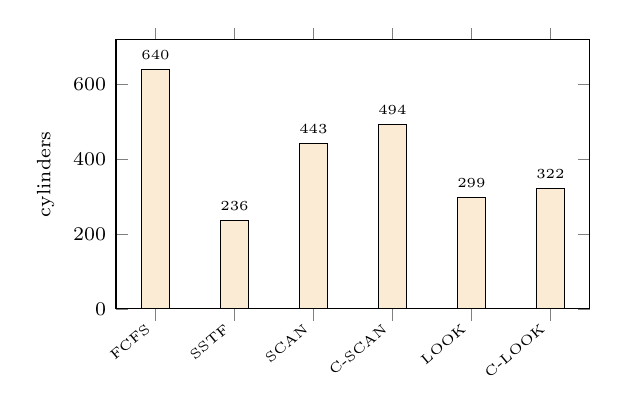
\begin{tikzpicture}
\begin{axis}[ybar, bar width=10pt, width=7.6cm, height=5cm, ymin=0, ymax=720,
  symbolic x coords={FCFS,SSTF,SCAN,C-SCAN,LOOK,C-LOOK}, xtick=data, xticklabel style={font=\tiny, rotate=40, anchor=east},
  ylabel={cylinders}, ylabel style={font=\scriptsize}, yticklabel style={font=\scriptsize},
  nodes near coords, nodes near coords style={font=\tiny}, enlarge x limits=0.1]
\addplot[fill=cStore, draw=black] coordinates {(FCFS,640) (SSTF,236) (SCAN,443) (C-SCAN,494) (LOOK,299) (C-LOOK,322)};
\end{axis}
\end{tikzpicture}
\caption{\texttt{disksim}: textbook queue 98 183 37 122 14 124 65 67, head 53}
\end{subfigure}\hfill
\begin{subfigure}{0.5\textwidth}\centering
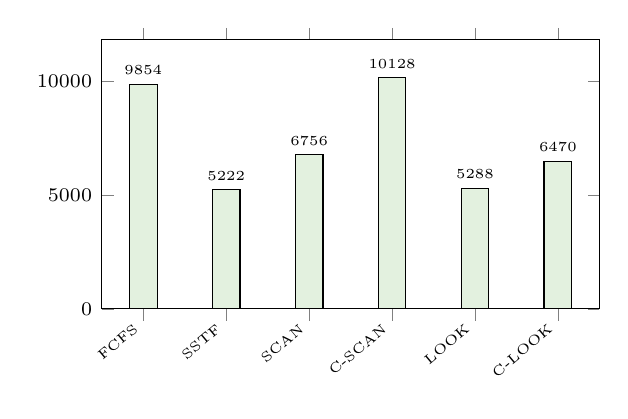
\begin{tikzpicture}
\begin{axis}[ybar, bar width=10pt, width=7.9cm, height=5cm, ymin=0, ymax=11800,
  symbolic x coords={FCFS,SSTF,SCAN,C-SCAN,LOOK,C-LOOK}, xtick=data, xticklabel style={font=\tiny, rotate=40, anchor=east},
  scaled y ticks=false, yticklabel style={font=\scriptsize, /pgf/number format/fixed, /pgf/number format/1000 sep={}},
  every node near coord/.append style={/pgf/number format/fixed, /pgf/number format/1000 sep={}},
  nodes near coords, nodes near coords style={font=\tiny}, enlarge x limits=0.1]
\addplot[fill=cKern, draw=black] coordinates {(FCFS,9854) (SSTF,5222) (SCAN,6756) (C-SCAN,10128) (LOOK,5288) (C-LOOK,6470)};
\end{axis}
\end{tikzpicture}
\caption{Measured: 125 requests from 5 concurrent \texttt{io} jobs}
\end{subfigure}
\caption{Total head movement of the six disk scheduling algorithms (TC10).}
\label{fig:disk}
\end{figure}

SSTF and LOOK move the head least. C-SCAN counts its return sweep to cylinder 0; with only five jobs the queue is short, so it pays that sweep often and on the live workload moves even more than FCFS, while giving every cylinder a more uniform waiting time.

\subsection{Memory, Page Replacement and Deadlock Avoidance Results}

\begin{figure}[H]
\centering
\begin{subfigure}{0.48\textwidth}\centering
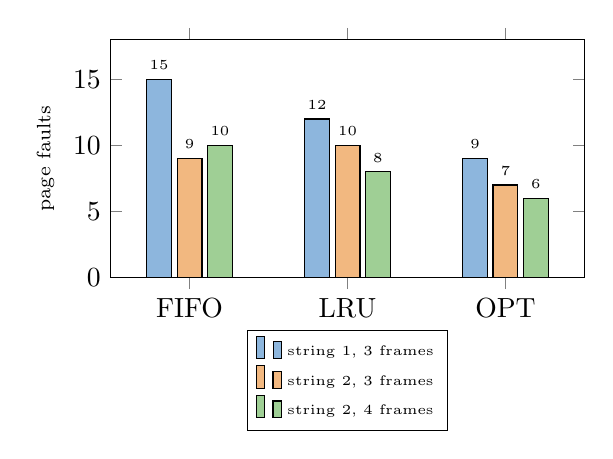
\begin{tikzpicture}
\begin{axis}[ybar, bar width=9pt, width=7.6cm, height=4.6cm, ymin=0, ymax=18,
  symbolic x coords={FIFO,LRU,OPT}, xtick=data, ylabel={page faults}, ylabel style={font=\scriptsize},
  legend style={font=\tiny, at={(0.5,-0.22)}, anchor=north, legend columns=1}, nodes near coords, nodes near coords style={font=\tiny}, enlarge x limits=0.25]
\addplot[fill=jA] coordinates {(FIFO,15) (LRU,12) (OPT,9)};
\addplot[fill=jB] coordinates {(FIFO,9) (LRU,10) (OPT,7)};
\addplot[fill=jC] coordinates {(FIFO,10) (LRU,8) (OPT,6)};
\legend{{string 1, 3 frames},{string 2, 3 frames},{string 2, 4 frames}}
\end{axis}
\end{tikzpicture}
\caption{\texttt{pagesim}; FIFO on string 2 shows Belady's anomaly}
\end{subfigure}\hfill
\begin{subfigure}{0.48\textwidth}\centering
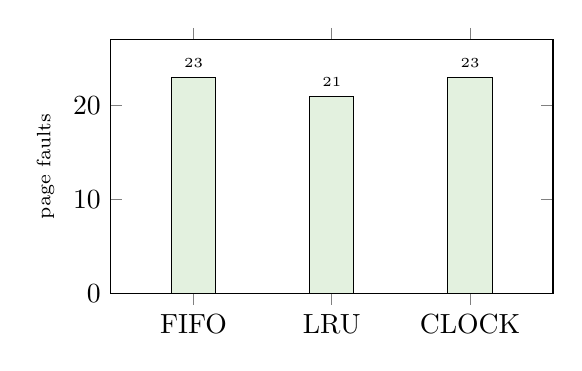
\begin{tikzpicture}
\begin{axis}[ybar, bar width=16pt, width=7.2cm, height=4.8cm, ymin=0, ymax=27,
  symbolic x coords={FIFO,LRU,CLOCK}, xtick=data, ylabel={page faults}, ylabel style={font=\scriptsize},
  nodes near coords, nodes near coords style={font=\tiny}, enlarge x limits=0.3]
\addplot[fill=cKern, draw=black] coordinates {(FIFO,23) (LRU,21) (CLOCK,23)};
\end{axis}
\end{tikzpicture}
\caption{Live page cache, 8 frames, 25 block reads}
\end{subfigure}
\caption{Page replacement results (TC9, TC11). String 1 = 7 0 1 2 0 3 0 4 2 3 0 3 2 1 2 0 1 7 0 1, string 2 = 1 2 3 4 1 2 5 1 2 3 4 5.}
\end{figure}

In TC8 five jobs claimed the classic maximums (7\,5\,3), (3\,2\,2), (9\,0\,2), (2\,2\,2), (4\,3\,3) against 10\,5\,7 resources. While they ran, \texttt{banker} reported the state as safe with sequence P2 P4 P1 P3 P5; one request that would have made the state unsafe was delayed, and all jobs finished without deadlock. The memory test (TC2) produced the map of Figure~\ref{fig:mem}, and jobs that did not fit correctly waited in the NEW state.

% ================= 9. REFERENCES =================
\section{References}

{\footnotesize\sloppy
\begin{enumerate}[label={[\arabic*]}, leftmargin=2.2em, itemsep=0pt]
  \item A. Silberschatz, P. B. Galvin and G. Gagne, \textit{Operating System Concepts}, 10th ed., Wiley, 2018.
  \item R. H. Arpaci-Dusseau and A. C. Arpaci-Dusseau, \textit{Operating Systems: Three Easy Pieces}, 2018. \url{https://pages.cs.wisc.edu/~remzi/OSTEP/}
  \item A. S. Tanenbaum and H. Bos, \textit{Modern Operating Systems}, 4th ed., Pearson, 2014.
  \item R. Cox, F. Kaashoek and R. Morris, \textit{xv6: a simple, Unix-like teaching operating system}, MIT. \url{https://pdos.csail.mit.edu/6.828/2023/xv6.html}
  \item E. W. Dijkstra, ``Een algorithme ter voorkoming van de dodelijke omarming,'' EWD 108, c.~1964 (the Banker's algorithm). \url{https://www.cs.utexas.edu/~EWD/transcriptions/EWD01xx/EWD108.html}
  \item P. J. Courtois, F. Heymans and D. L. Parnas, ``Concurrent control with `readers' and `writers','' \textit{Comm. ACM}, 14(10), 1971.
  \item L. A. Belady, ``A study of replacement algorithms for a virtual-storage computer,'' \textit{IBM Systems Journal}, 5(2), 1966.
  \item L. A. Belady, R. A. Nelson and G. S. Shedler, ``An anomaly in space-time characteristics of certain programs running in a paging machine,'' \textit{Comm. ACM}, 12(6), 1969.
  \item The Linux man-pages project: \texttt{makecontext(3)}, \texttt{setitimer(2)}, \texttt{sigprocmask(2)}, \texttt{pthread\_cond\_wait(3p)}. \url{https://man7.org/linux/man-pages/}
\end{enumerate}
}

\end{document}
